\documentclass{article}
\usepackage{arxiv}
\usepackage[utf8]{inputenc} % allow utf-8 input
\usepackage{svg}
\usepackage{indentfirst}
\usepackage[T1]{fontenc}    % use 8-bit T1 fonts
\usepackage{hyperref}      % hyperlinks
\usepackage[none]{hyphenat}
\usepackage{tikz}
\usetikzlibrary{quantikz2}
\usepackage{listings}
\usepackage{url}            % simple URL typesetting
\usepackage{booktabs}       % professional-quality tables
\usepackage{amsfonts}       % blackboard math symbols
\usepackage{nicefrac}       % compact symbols for 1/2, etc.
\usepackage{microtype}      % microtypography
\usepackage{lipsum}		% Can be removed after putting your text content
\usepackage{graphicx}
\usepackage{doi}
\usepackage{authblk}
\usepackage{framed,multirow}
%% The amssymb package provides various useful mathematical symbols
\usepackage{amssymb}
\usepackage{latexsym}
\usepackage{graphicx}
\usepackage{amsmath}
\usepackage{booktabs} % for better looking tables
\usepackage{tabularx}
\usepackage{array}
\usepackage{etoolbox}
\usepackage{subcaption}
\usepackage{algorithm}
\usepackage{algorithmic}
\usepackage{indentfirst}
\usepackage{authblk}
\usepackage{float}
\usepackage[nameinlink, noabbrev]{cleveref} % Load cleveref after hyperref
% Define the format and colors for different reference types
\crefformat{figure}{#2{\color{red}Figure~#1}#3}
\crefformat{section}{#2{\color{red}Section~#1}#3}
\crefformat{equation}{#2{\color{red}Equation~#1}#3}
\crefformat{table}{#2{\color{red}Table~#1}#3}
\crefformat{algorithm}{#2{\color{red}Algorithm~#1}#3}
% Following three lines are needed for this document.
% If you are not loading colors or url, then these are
% not required.
\usepackage[table]{xcolor}
% Define a new centered column type with a fixed width
\newcolumntype{C}[1]{>{\centering\arraybackslash}p{#1}}
% Define a new centered column type for tabularx
\newcolumntype{H}{>{\centering\arraybackslash}X}
\usepackage{enumitem}
\newlist{boldenum}{enumerate}{1}
\setlist[boldenum]{label=\textbf{(\arabic*)}}
\definecolor{newcolor}{rgb}{.8,.349,.1}
\newcommand{\nonumfootnote}[1]{
    \begingroup
    \renewcommand\thefootnote{}
    \footnotetext{#1}
    \endgroup
}

\title{\Large A novel approach of secure audio transmission in Post-quantum Era.}
%\date{September 9, 1985}	% Here you can change the date presented in the paper title
%\date{} 					% Or removing it
\author[2]{\large Md. Raisul Islam Rifat}
\author[1]{\large Md. Mizanur Rahman}
\author[2]{\large Md. Abdul Kader Nayon}
\author[3, *]{\large M.R.C. Mahdy}
\affil[1]{Department of CSE, RUET}
\affil[2]{Department of EEE, CUET}
\affil[3]{Department of Electrical and Computer Engineering, North South University, Bashundhara, Dhaka}
% Uncomment to remove the date
%\date{}
% Uncomment to override  the `A preprint' in the header
%\renewcommand{\headeright}{Research Article}
%\renewcommand{\undertitle}{Research Article}
%\renewcommand{\shorttitle}{\textit{Research Article}}
%%% Add PDF metadata to help others organize their library
%%% Once the PDF is generated, you can check the metadata with
%%% $ pdfinfo template.pdf
% \hypersetup{
% pdftitle={A template for the arxiv style},
% pdfsubject={q-bio.NC, q-bio.QM},
% pdfauthor={David S.~Hippocampus, Elias D.~Striatum},
% pdfkeywords={First keyword, Second keyword, More},
% }

\begin{document}
%\emergencystretch 3em

\maketitle


\begin{abstract}
\end{abstract}
\lipsum[1]
% keywords can be removed
\keywords{Lorem ipsum, Placeholder text, Text generation, Typography, LaTeX formatting, Document design, Content management, Semantic analysis, Latin text, Formatting templates, Filler content, Automated writing, Document structure
}

% Corresponding Author footnote
\nonumfootnote{* Corresponding author.
    \textit{E-mail address}: \href{mahdy.chowdhury@northsouth.edu}{mahdy.chowdhury@northsouth.edu} (M.R.C. Mahdy).}

% hold ctrl & / to comment a line or paragraph.


\section{Introduction}
\label{sec:introduction}
The simplest, as well as the most important, form of exchange for human beings is verbal communications. The invention of the Telephone by Alexander Graham Bell in 1876 transformed the verbal communication demography - making the transmission of human voice, which are essentially audio signals, over long distances possible. In the subsequent centuries, technological improvements has broadened the scope of audio transmission. With the rise of the Internet, the amount of information exchanged through audio signals increased rapidly. This increase number audio transmission resulted in the development of different encryption techniques and cryptographic algorithms. The most popular among these algorithms are the symmetric AES and the asymmetric RSA encryption schemes. AES \cite{rijmen2001advanced} is a block cipher scheme that utilizes multiple matrix operation to encrypt and decrypt data using the same key. Without any knowledge of the cipher key, it is computationally infeasible to reverse the orations performed during encryption. RSA \cite{rivest1978method}, on the other hand, utilizes prime number factorization to generate public-private key-pairs for each user that are used to encrypt and decrypt data. The security of the RSA scheme relies on the insane amount of computational power required to obtain the private key from a public through prime number factoring.

However, with the advent of Quantum Computers with increasing number of functional qubits, these classical cryptography and encryption schemes face an imposing threat \cite{bernstein2017post}. In 1996, Lov K. Grover proposed an algorithm to search an unordered database of size $N$ using $\sqrt{N}$ quantum queries \cite{grover1996fast}. Using Grover's algorithm, the number of trials required to brute-force a key of length $k$ reduces from $2^{k}$ to $2^{k/2}$. This reduction in number of brute-force trials effectively reduces the security level of symmetric encryption schemes such as AES \cite{Daemen2002}. For example, the AES-128 encryption scheme with a pre-quantum security level of 128 reduces to a post-quantum security level of 64, which is much easier to brute-force. In 1994, P.W. Shor presented a quantum algorithm that can quickly find the prime factorization of any positive integer $N$ \cite{Shor1997}. As the security of the RSA algorithm relies on the arduousness of prime number factorization to derive private key from public key, it is currently facing an existential threat due to the exponential speed of Shor's algorithm. It is estimated that the time complexity for Shor' algorithm is $\mathcal{O}(72(log(N))^{3})$, as opposed to $\mathcal{O}(N^3)$ for classical computers.

To address these arising challenges, new research is being done on the field of quantum augmented communication systems. These systems exploits the principles of quantum mechanics to attain secure data transmission. One of the most promising area of research in the field of quantum communications is Quantum Key Distribution (QKD). QKD protocols works by establishing a secure cryptographic key between two users over an insecure channel \cite{alleaume2014using}. QKD employ properties unique to quantum mechanics, such as the no-cloning theorem \cite{buvzek1996quantum} and the uncertainty principle \cite{sen2014uncertainty}, that ensures the detection of any eavesdropping attempts and thereby guarantees the security of the key. However, QKD itself does not provide security on its own, rather it facilitates the establishment and secure exchange of secret keys that are subsequently used by other cryptographic algorithms and encryption techniques to secure the transmitted information. In resemblance, the research being done on the field of steganography heralds the emergence of an effective information concealing technique to obscure sensitive information within seemingly harmless transmission. Steganography is the technique of hiding secret massage within another massage in such a manner that it is not discernible that a secret message is embedded \cite{Kahn1996}. However, the security of any steganographic technique is heavily dependent on the strength of cryptographic technique employed to encrypt the data \cite{anderson1998limits}.

This paper introduces a novel approach to reinforce the security of digital audio communication by combining the competency of QKD, classical encryption schemes and steganography. Our system utilizes the E91 QKD protocol proposed by Artur K. Ekert in 1991 \cite{Ekert1991} to generate a shared key with increased security, which is then hashed to produce a fixed-length (256 bits), high-entropy key that is suitable for symmetric encryption by employing the Secure Hashing Algorithm-3 (SHA3-256) \cite{dworkin2015sha}. We inspect the use of ChaCha20-Poly1305 authenticated encryption with associated data (AEAD) algorithm \cite{rfc7539} - which combines the stream cipher scheme, ChaCha20 \cite{bernstein2008chacha} with the message authentication code, Poly1305 \cite{bernstein2005poly1305} - to encrypt the steganographic audio. We performed least significant bit (LSB) substitution steganography to hide an audio signal inside another audio signal \cite{cvejic2002increasing}. The incorporation of QKD with classical symmetric encryption addresses various security concernment, providing protection against both classical and quantum threats.

The new vulnerabilities in secure data transmission due to quantum computer and the need to oppose them have been the motivation for our research. With the advancement in quantum computing technology, it is imperative to devise innovative cryptographic techniques that can keep the data secure in the prospect of an attack from these powerful computers. It is our aim to develop a vigorous solution for secure data communication by combining the strength of quantum communication with hash function, classical encryption and steganography. Hence, the objective our experimental work is to investigate the viability and credibility of integrating encrypted steganographic techniques with quantum protocols, specifically QKD, to strengthen the security and resilience of audio communication. This innovative amalgamation of steganography and quantum communication embodies a significant furtherance in the field, providing an exceptional and optimistic approach to secure data transmission. Our main contribution can be summarized as follows -
\begin{itemize}
    \item Proposed an original architecture that successfully combines E91 QKD protocol, ChaCha20-Poly1305 AEAD and audio steganography using LSB.
    \item Utilized E91 as the key distribution protocol which employs principles of quantum mechanics for secure key exchange.
    \item Assimilated audio steganography using LSB substitution into the architecture to augment the security and robustness of the overall system.
    \item Assessed the performance and reliability of the proposed scheme by measuring the security through end-to-end encryption.
\end{itemize}

Our paper is organized is as follows - Section \ref{sec:relatedWorks} demonstrates the present sate of the field through the review of existing research and their development, laying the foundation for our our proposed scheme. Section \ref{sec:preliminaries} describes the foundational concepts of our proposed schemes. Section \ref{sec:methodology} describes the proposed methodology, presenting a detailed piecemeal explanation of our proposed architecture. In section \ref{sec:experminats}, we present the experimental methods as well as the findings. Section \ref{sec:discussion} explore deeper into an extensive analysis of the results, construing the findings and excerpting key insights. Finally, section \ref{sec:conclusion} concludes the paper by indicating the direction of future work, highlighting the potential application and extension of our research.
\section{Related Works}
\label{sec:relatedWorks}

\section{Preliminaries}
\label{sec:preliminaries}
\subsection{Ekert 91 Protocol}
\label{sec:e91}
The E91 protocol is a quantum key distribution (QKD) scheme that uses entangled photon pairs and the violation of Bell's inequality to securely distribute cryptographic keys between two parties, typically referred to as Alice and Bob.
The Ekert91 protocol, based on the principles of quantum mechanics and entanglement, allows secure key distribution between two parties, Alice and Bob. The steps are as follows:

\begin{enumerate}
    \item Alice and Bob exchange several entangled Bell states, $\ket{\psi^{-}_{AB}}$, where Alice holds the first subsystem and Bob holds the second.
    \item For each entangled state, they independently and randomly select a measurement direction from their respective sets $\{A_i\}$ and $\{B_i\}$.
    \item After completing the measurements, Alice and Bob publicly share their chosen measurement bases. When their bases align (i.e., $(A_1, B_1)$ and $(A_3, B_3)$), the corresponding measurement outcomes are used to construct the sifted key.
    \item The measurement outcomes from mismatched bases, such as $(A_1, B_3)$, $(A_1, B_2)$, $(A_2, B_3)$, and $(A_2, B_2)$, are analyzed to verify the violation of the CHSH inequality.
    \item Finally, Alice and Bob perform error correction and privacy amplification processes to transform the sifted key into a secure shared secret key.
\end{enumerate}

A source, usually referred to as Charlie, generates entangled photon pairs in a singlet state:
\[\ket{\psi^{-}_{AB}} = \frac{1}{\sqrt{2}}\left(\ket{01}_{AB}-\ket{10}_{AB}\right)
\]
where $\ket{0}$ and $\ket{1}$ represent the two possible polarization states of the photons.
\begin{figure}[!h]
    \includesvg[width=\textwidth]{measurement.svg}
    \caption{Direction of measurement for Ekert Protocol}
    \label{fig:ekertMeasurement}
\end{figure}

In the Ekert protocol, Alice and Bob each perform a random measurement on their respective parts of the entangled state. For each of these bipartite states $\ket{\psi^{-}_{AB}}$, they choose an observable from two sets, $\{A_i\}$ for Alice and $\{B_i\}$ for Bob. These observables correspond to spin components in the x-z plane of the Bloch sphere, as shown in \ref{fig:ekertMeasurement}. The measurement directions are defined by the angles $\varphi_A$ and $\varphi_B$ for Alice and Bob, respectively.

The measurement operators for Alice and Bob are given by:
\[
    A_i = \cos(\varphi_A^i) + \sin(\varphi_A^i) \quad \text{for Alice, and} \quad B_i = \cos(\varphi_B^i) + \sin(\varphi_B^i) \quad \text{for Bob.}
\]
Here, $Z=\ket{0}\bra{0}-\ket{1}\bra{1}$ and $X=\ket{+}\bra{+}-\ket{-}\bra{-}$ are the Pauli operators for the measurement.

For Alice, the angles are defined as:
\[
    \varphi_A^1 = 0, \quad \varphi_A^2 = \frac{\pi}{2}, \quad \varphi_A^3 = \frac{\pi}{4}.
\]
For Bob, the angles are:
\[
    \varphi_B^1 = 0, \quad \varphi_B^2 = -\frac{\pi}{4}, \quad \varphi_B^3 = \frac{\pi}{4}.
\]

In terms of the measurement operators, these can be expressed as:
\[
    A_1 = Z, \quad A_2 = X, \quad B_1 = Z, \quad B_2 = \frac{1}{\sqrt{2}} (Z - X), \quad A_3 = \frac{1}{\sqrt{2}} (Z + X), \quad B_3 = \frac{1}{\sqrt{2}} (Z + X).
\]

It is important to note that the measurements $A_1$ and $B_1$, as well as $A_3$ and $B_3$, are those where Alice and Bob choose the same measurement direction. These measurement choices are crucial for the key generation process, as they result in correlated outcomes that form the sifted key.

In the next step, Alice and Bob announce the directions of their measurements. When their measurement directions match, such as $(A_1 , B_1)$ and $(A_3 , B_3)$, their results are perfectly anti-correlated. By flipping all the bits for one of them, they can generate the sifted key. The results from other combinations of measurements, like $(A_1 , B_3), (A_1 , B_2), (A_2 , B_3), \text{and} (A_2 , B_2)$, are used to assess how much an eavesdropper might know about the key. This is done by checking the CHSH inequality, a classical correlation bound that is part of the Bell inequalities. The CHSH inequality involves four random variables \( A1, A2, B2, B3 \), each taking values of \( +1 \) or \( -1 \). By evaluating these random variables, the inequality states that the sum of certain correlations must not exceed 2.

% In the quantum case, the measurement operators for \( A1, A2, B2, B3 \) are treated as quantum observables. The expectation values of their products are calculated using the state \( \rho = \ket{\psi^{-}}\). For example, the expectation value of \( A1B3 \) is found to be $\displaystyle  -\frac{1}{\sqrt{2}} $. By computing the sum of all these expectation values, we obtain a value of
% \[
% S = \frac{2}{\sqrt{2}},
% \]
% which violates the CHSH inequality. This indicates that Alice and Bob share a maximally entangled state, and there is no information about the key that an eavesdropper could gain. If \( S \leq 2 \), it means the states are separable, and no secret key can be generated.
The remaining measurement results are used to generate a shared secret key. Only the measurement results obtained along compatible axes are used to establish the key.

The security of the E91 protocol is derived from the following principles:
\begin{itemize}
    \item \textit{Quantum Entanglement}: Any attempt at eavesdropping would disturb the entangled state, leading to detectable anomalies in the correlations.
    \item \textit{Bell's Inequality}: The violation of Bell's inequality rules out classical explanations for the correlations, ensuring the integrity of the quantum channel.
\end{itemize}

By utilizing the properties of quantum entanglement, the E91 protocol achieves an unprecedented level of security, making it a cornerstone in the field of quantum cryptography.
\subsection{SHA3 -- 256 Hash Function}
\label{sec:sha3}
SHA-3 is the latest member \cite{nistHashFunctions} of the Secure Hash Algorithm (SHA) family of cryptographic hash functions. Based on the K\textsc{eecak} algorithm \cite{Bbbbbbb2011}, the SHA-3 standard differs fundamentally from it's MD-5 \cite{rivest1992md5} like structured predecessors -- SHA-1 and SHA-2 \cite{penard2008secure}. In its essence, the SHA-3 standard is a hash function, that is, for any length of binary data input, there is an output of fixed length. The output is called the \textit{digest} or \textit{hash value}. Depending on the digest length, the four hash functions are called SHA3-224, SHA3-256, SHA3-384 and SHA3-512. The suffixes after the dash indicate the fixed length of the digest, for example, SHA3-256 - which is of interest to our methodology - produces 256 bits long digest. As the digest length is constant irrespective of input length, SHA3 is ideal for integrity and signature verification, as well as password hashing, that is not storing password in clear-text format, rather storing the hash of the password for verification.

SHA-3 works by using the sponge construction \cite{keccakKeccakTeam}. Here, data is "absorbed" into the sponge and the result is "squeezed" out, as sown in Figure \ref{fig:sponge}. For an input bit string $N$, a padding function $pad$, and a permutation function $f$ yields the spnge construction $Z=\text{sponge}[f,pad,r](N,d)$. Here, the permutation function $f$ operates on a bit block of width $b$, rate $r$ and yields and output of length $d$. From the sponge construct, we have capacity $c=b-r$ and digest $Z$ of length $b$. The block permutation $f$ is Keccak-f[1600] that utilizes XOR, AND and NOT operations. It is defined for any power-of-two word size, $w=2^l$. The basic block permutation function consists of $12+2l$ rounds of five steps: $\theta$ (parity computation), $\rho$ (bitwise rotation), $\phi$ (permuatation), $\chi$ (bitwise combination) and $\iota$ (XOR).

\begin{figure}[!h]
    \centering
    \includesvg[width=\textwidth]{SpongeConstruction.svg}
    % 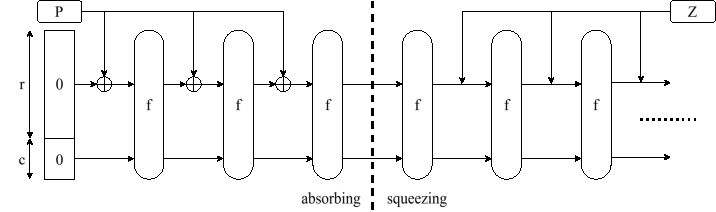
\includegraphics[width=0.75\textwidth]{SpongeConstruction.pdf}
    \caption{The sponge construction for SHA-3.}
    \label{fig:sponge}
\end{figure}

The process of retrieving the digest $Z$ from input $N$ is described below --
\begin{itemize}
    \item The input $N$ is padded using the padding function, $pad$. This yields in a padded bit strength $P$ the length of which is devisable by $r$ ($n=\text{len}(P)/r$).
    \item $P$ is broken into $n$ consecutive pieces, each piece of length $r$, so that $P \to P_{0},\ldots,P_{n-1}$
    \item State $S$ is initialized with sting of $b$ zero bits.
    \item The input is absorbed into the state: for each block $P_{i}$, \begin{itemize}
              \item $P_{i}$ is extended at the end by $c$ zero bits, so that the length is $b$.
              \item The resulting bit string is XORed with $S$.
              \item The block permutation $f$ is applied on the result, yielding a new state $S$.
          \end{itemize}
    \item $Z$ is initialized with empty string
    \item while \textit{length}$(Z)<d$:\begin{itemize}
              \item The first $r$ bits of $S$ is appended to $Z$.
              \item \textit{if} $(\textit{length}(Z)<d)$, apply $f$ to $S$, yielding a new $S$.
          \end{itemize}
    \item $Z$ is truncated to $d$ bits.
\end{itemize}

For example, for the following binary stream, $N=$
\subsection{ChaCha20-Poly1305}
\label{sec:chacha20}
ChaCha20-Poly1305 is an authenticated encryption with associated data (AEAD) algorithm that provides a comparatively fast software performance. It is typically faster than AES-GCM (Galois/Counter Mode) in the absence of hardware acceleration \cite{rfc7539}. This algorithm combines the ChaCha20 stream cipher \cite{bernstein2008chacha} and the Poly1305 \cite{bernstein2005poly1305} universal hash family that acts as message authentication code -- both of which was developed independently by Daniel J. Bernstein.

A stream cipher is a symmetric key cipher, that is an encryption and decryption algorithm, that combines plaintext data with a pseudorandom keystream \cite{robshaw1995stream}. Stream ciphers works by encrypting each plaintext digit one at a time with the corresponding keystream digit, as opposed to block ciphers where blocks of plaintext with a certain length is encrypted with the keystream. In 2008, Bernstein proposed the ChaCha family of stream ciphers, a successor to the Salsa20 stream cipher \cite{bernstein2005salsa20} proposed by Bernstein in 2005. ChaCha was proposed as an alternative to Salsa20 \cite{bernstein2008chachaFamily} with slightly better performance. Similar to it's predecessor, the initial state of ChaCha is 512-bit long -- made up of a 128-bit constant, a 256-bit key, a 64-bit counter and a 64-bit nonce. The 128-bit constant is usually \textit{"expand 32-byte k"}. This 512-bit long input is arranged in a $4\times4$ matrix where each entry is a 32-bit word. The matrix arrangement is shown bellow --
\begin{equation}\label{initialState}
    \left[
        \begin{array}{cccc}
            \text{Consant}[0] & \text{Consant}[1] & \text{Consant}[2] & \text{Consant}[3] \\
            \text{Key}[0]     & \text{Key}[1]     & \text{Key}[2]     & \text{Key}[3]     \\
            \text{Key}[4]     & \text{Key}[5]     & \text{Key}[6]     & \text{Key}[7]     \\
            \text{Conter}[0]  & \text{Conter}[1]  & \text{Nonce}[0]   & \text{Nonce}[1]
        \end{array}
        \right]
\end{equation}
The core operation of ChaCha, and it's predecessor Salsa20, is the quarter-round \text{\ttfamily{QR(a,b,c,d)}}. ChaCha uses 4 additions, 4 XORs and 4 rotations to update 4 32-bit state words -- \text{\ttfamily{a,b,c,d}}. The update procedure is as follows --
\begin{lstlisting}[basicstyle=\ttfamily,frame=none]
    a += b; d ^= a; d <<<= 16;
    c += d; b ^= c; b <<<= 12;
    a += b; d ^= a; d <<<=  8;
    c += d; b ^= c; b <<<=  7;
\end{lstlisting}

If the elements of matrix \ref{initialState} is indexed from 0 to 15
\[\left[
        \begin{array}{cccc}
            0  & 1  & 2  & 3  \\
            4  & 5  & 6  & 7  \\
            8  & 9  & 10 & 11 \\
            12 & 13 & 14 & 15
        \end{array}
        \right]\]
a double round in ChaCha is defined as --
\begin{lstlisting}[basicstyle=\ttfamily,frame=none]
    // Odd round
    QR(0, 4,  8, 12) // column 1
    QR(1, 5,  9, 13) // column 2
    QR(2, 6, 10, 14) // column 3
    QR(3, 7, 11, 15) // column 4
    // Even round
    QR(0, 5, 10, 15) // diagonal 1 (main diagonal)
    QR(1, 6, 11, 12) // diagonal 2
    QR(2, 7,  8, 13) // diagonal 3
    QR(3, 4,  9, 14) // diagonal 4
\end{lstlisting}
ChaCha20 uses 10 iterations of the double round -- an overall of 20 rounds. Hence the name ChaCha20.

Each word is updated twice in ChaCha20's quarter rounds, as opposed to Salsa20 where each word is updated only once. This results in an average of $12.5$ output bits to change in each quarter round of ChaCha20, while the Salsa20 quarter-round changes 8 output bits. Although the ChaCha quarter round contains the same number of adds, xors, and bit roattes as the Salsa20 quarter round, it is slightly fatser because two of the roate functions are multiples of 8, allowing for a small optimization for x86 and other architectuires.

After the 10 iterations, a keystream, $K$ is generated which is XORed with the message stream, $M$, to produce the cipher, C.
\[C = K \oplus M\]
For decryption, the keystream, $K$, is XORed with the cipher, $C$, to retrieve the message, $M$.
\[M = C \oplus K\]
\begin{figure}[!h]
    \centering
    \includesvg[width=\textwidth]{ChaCha_Cipher_Quarter_Round_Function.svg}
    \caption{The ChaCha quarter-round function.}
\end{figure}

A hash function is a special mathematical function that can data of arbitrary size to constant-sized values. The output of a hash function is called hash digest or simply hashes. A unique property of most hash functions is their ability to generate unique digests for each unique inputs. This makes hash functions invaluable for authentication and data integrity verification.In 2002, Bernstein designed the Poly1305 universal hash function, which was intended to provide a message authentication code to authenticate a message using a shared secret key \cite{bernstein2005protecting}. The original implementation of Poly1305 was in 2005 when Poly1305 hash was combined as a Carter-Wegman authenticator \cite{carter1981new} with AES-128 to authenticate encrypted messages.

Poly1305 provides a 128-bit long authentication tag from a 256-bit long one-time key, and a message of arbitrary length. The key has two portions -- $r$ and $s$. It is recommended that the pair $(r,s)$ to be unique. The first portion, $r$, is a 128-bit key produced form a symmetric encryption scheme similar to AES. The later portion, $s$, is a 128-bit long integer arranged as a 16-octet little-endian format. It is required that --
\begin{itemize}
    \item $r[3], r[7], r[11]$ and $r[15]$ have their top four bits clear (to be in $\{0,1,\ldots,15\}$).
    \item $r[4], r[8]$ and $r[12]$ have their bottom four bits clear (to be in $\{0,4,8,\ldots,252\}$).
\end{itemize}

Each message is required to accompanied by a 128-bit Nonce generated from the accompanying encryption scheme. The process of producing the authenticator tag from the message and the key are briefly outlined here --
\begin{itemize}
    \item A variable called the "accumulator" is initialized with zeros
    \item The message is divided into 128-bit long blocks. Each block is read in little-endian sequence.
    \item Each block is appended by 1 byte so that each block is 136-bit long. If any of the block is not 136-bit long (usually the last block), the block is padded with zeros to make it of proper length.
    \item Each 136-bit long message block is multiplied with a clamped value $r$ and the multiplication result is added to the accumulator.
    \item The value stored in the accumulator is reduced using $mod(2^{128})$ and the reduced value is stored in the accumulator.
    \item When the whole message is converted, the value in the accumulator is added to $s$.
    \item From the result, the 128 least significant bits are formatted in little-endian format to produce the tag.
\end{itemize}

The ChaCha20-Poly1305 AEAD adopted for Internet Engineering Task Force (IETF) \cite{rfc8439} and subsequently as the standard for Transport Layer security (TLS) \cite{rfc7905} and the OpenBSD Secure Shell (OpenSSH) \cite{miller2015chacha20} is slightly different from the original structures proposed by Daniel J. Bernstein. To be precise, the ChaCha20 symmetric encryption is slightly modified. As opposed to a 64-bit Nonce, the modified ChaCha20 has a 96-bit long Nonce. The modified matrix is shown below --
\begin{equation}\label{initialStateMod}
    \left[
        \begin{array}{cccc}
            \text{Consant}[0] & \text{Consant}[1] & \text{Consant}[2] & \text{Consant}[3] \\
            \text{Key}[0]     & \text{Key}[1]     & \text{Key}[2]     & \text{Key}[3]     \\
            \text{Key}[4]     & \text{Key}[5]     & \text{Key}[6]     & \text{Key}[7]     \\
            \text{Conter}[0]  & \text{Nonce}[0]   & \text{Nonce}[1]   & \text{Nonce}[2]
        \end{array}
        \right]
\end{equation}

The remaining portions of the ChaCha20 scheme remains unaltered. The same is true for the Poly1305 authenticator. A high level overview of this modified ChaCha20 encryption and Poly1305 authenticator tag generation is outlined below --
\begin{itemize}
    \item A 256-bit long string is used as key for the ChaCha20 key along with a unique 96-bit long Nonce.
    \item Using the key and the nonce, the ChaCha20 block function is activated, which produces a 512-bit state.
    \item The first 256 serialized bits of the 512-bit state is taken as the Poly1305 key -- the 128 bit as $r$ and the next 128 bit as $s$.
    \item The 512-bit state is serialized in little-endian format to produce a keystream.
    \item The keystream is XORed with the message to produce the ciphertext.
    \item The Poly1305 function is called with the ciphertext and the previously derived key as input to produce the authenticator tag.
\end{itemize}
The output from the AEAD is the concatenation of the following --
\begin{itemize}
    \item A ciphertext which is as long as the plaintext message.
    \item A 128-bit authenticator tag, generated by the Poly1305 function.
\end{itemize}
\subsection{LSB Steganography}
\label{sec:steganography}
Steganography is the process where we don't encrypt the secrete message, rather we hide it in another file. Trough this process we can hide different types of secrete data like text, image, video, audio etc. within cover data which can also be in any different data types.\cite{jayaram2011information}\cite{hemeida2021comparative}
\begin{figure}[H]
    \begin{center}
        \includesvg[width=\textwidth]{steganographyApplication.svg}
        \caption{Steganography Application Scenario}
        \label{fig:stegoApplication}
    \end{center}
\end{figure}

In Audio Steganography secret message is hidden in cover audio but there is no much change in the cover audio because it is it use of the psycho-acoustical masking phenomenon of the human auditory system(HAS). There are different methods of steganography. Among them some notables are: LSB Coding, Parity Coding, Phase coding, Spread sprectrum, Echo hiding etc.\cite{hemeida2021comparative} A very popular methodology among them is the LSB(Least Significant Bit) algorithm, which only replaces the least significant bits of the some of the bytes of the cover audio. Due to LSB substitution there is no much changes in the audio also.
\begin{figure}[!h]
    \begin{center}
        \includesvg[width=\textwidth]{embedStego.svg}
        \caption{Block Diagram of LSB Embedding implementation logic.}
        \label{fig:stegoEmbed}
    \end{center}
\end{figure}

LSB encoding embeds secret audio by replacing the least significant bits of carrier audio frames with bits from the secret audio. First, the carrier and secret audio are checked for compatibility in terms of channels and sample width. The secret audio frames are resized to fit the carrier’s capacity. A mask is applied to clear the carrier’s LSBs, which are then replaced with shifted bits from the secret audio. The result is a modified carrier audio with embedded data, saved as a new file.
\begin{figure}[!h]
    \begin{center}
        \includesvg[width=\textwidth]{extractStego.svg}
        \caption{Block Diagram for Steganalysis for extracting the embedded data.}
        \label{fig:stegoExtract}
    \end{center}
\end{figure}

Decoding isolates the embedded bits by applying a mask on the embedded audio and shifting these bits back to their original positions to reconstruct the secret audio. To improve quality, a low-pass filter reduces noise. The reconstructed audio is clipped to valid ranges and saved as the extracted secret.
\section{Methodology}
\label{sec:methodology}
The architecture that we proposed is a system that integrates E91 QKD protocol with classical cryptographic schemes and lsb steganography to ensure a heavily secure audio data encryption system. The system utilizes the E91 for QKD to generate and exchange the cryptographic keys called the Ekert key, SHA3 to derive a high-entropy 256-bit key from the Ekert key for ChaCha20-Poly1305 encryption and LSB substitution for steganography. The architecture ensures augmented data security through the combination of classical and quantum techniques. Figure \ref{fig:methodology} provides a high level overview of our proposed system.
\begin{figure}[!h]
    \begin{center}
        \includesvg[width=\textwidth]{methodology.svg}
        \caption{Methodology}
        \label{fig:methodology}
    \end{center}
\end{figure}
\subsection{Initialization}
\label{sec:init}
As outlined by Ekert \cite{Ekert1991}, an entangled pair generator, referred to as Charlie, produces pairs of entangled qubits and shares them with Alice and Bob. The circuit shown in Figure \ref{fig:singlet} is used to produce the entangled qubit pairs. The circuit applied a Hadamard $(H)$ gate to put a qubit in superposition and a CNOT $(\oplus)$ gate to control the other qubit. Here, $qr_{0}$ and $qr_{1}$ denotes quantum registers, that is, qubits, while $cr$ denotes classical register.
\begin{figure}[!h]
    \centering
    \begin{quantikz}
        \lstick{$qr_{0}$} & \gate{H} & \ctrl{1} & \\
        \lstick{$qr_{1}$} & & \targ{} &  \\
        \lstick{$cr$}\setwiretype{c} & & &
    \end{quantikz}
    \caption{Singlet circuit for creating entanglement qubit pairs.}
    \label{fig:singlet}
\end{figure}
\subsection{Measurement}
\label{sec:measurement}
Alice and Bob independently create a random set of bases of length $n$. Using this set of random bases, Alice and Bob perform measurements on the qubits they received from Charlie. The respective measurement circuits are shown in Figures \ref{fig:aliceMeasurements} and \ref{fig:bobMeasurements}. After the completion of the measurements, both parties share their measurement bases over an unsecured Classical Channel. Upon comparison of these measurement bases, the states that lack a common base are discarded. The result is a secret key called the Final Ekert Key that is shared between Alice and Bob. The measurement process is illustrated in Figure \ref{fig:combined}.
\begin{figure}[!h]
    \begin{subfigure}[h]{0.5\textwidth}
        \centering
        \begin{quantikz}
            \lstick{$qr_{0}$} & \gate{S} & \gate{H} & \gate{T} & \gate{H} & \meter{} \wire[d][2]{c} & \\
            \lstick{$qr_{1}$} & & & & & & \\
            \lstick{$cr$}\setwiretype{c} & & & & & &
        \end{quantikz}
        \caption{$W$ basis}
    \end{subfigure}
    \hfill
    \begin{subfigure}[h]{0.5\textwidth}
        \centering
        \begin{quantikz}
            \lstick{$qr_{0}$} & \gate{H} & \ctrl{1} & \meter{} \wire[d][2]{c} & \\
            \lstick{$qr_{1}$} & & \targ{} & & \\
            \lstick{$cr$}\setwiretype{c} & & & &
        \end{quantikz}
        \caption{$X$ basis}
    \end{subfigure}
    \vfill
    \begin{subfigure}[h]{\textwidth}
        \centering
        \begin{quantikz}
            \lstick{$qr_{0}$} & \meter{} \wire[d][2]{c} & \\
            \lstick{$qr_{1}$} & & \\
            \lstick{$cr$}\setwiretype{c} & &
        \end{quantikz}
        \caption{$Z$ basis}
    \end{subfigure}
    \caption{Alice's measurement circuits.}
    \label{fig:aliceMeasurements}
\end{figure}
\begin{figure}[!h]
    \begin{subfigure}[h]{0.5\textwidth}
        \centering
        \begin{quantikz}
            \lstick{$qr_{0}$} & & & & & & \\
            \lstick{$qr_{1}$} & \gate{S} & \gate{H} & \gate{T^\dag} & \gate{H} & \meter{} \wire[d][1]{c} & \\
            \lstick{$cr$}\setwiretype{c} & & & & & &
        \end{quantikz}
        \caption{$V$ basis}
    \end{subfigure}
    \hfill
    \begin{subfigure}[h]{0.5\textwidth}
        \centering
        \begin{quantikz}
            \lstick{$qr_{0}$} & & & & & & \\
            \lstick{$qr_{1}$} & \gate{S} & \gate{H} & \gate{T} & \gate{H} & \meter{} \wire[d][1]{c} & \\
            \lstick{$cr$}\setwiretype{c} & & & & & &
        \end{quantikz}
        \caption{$W$ basis}
    \end{subfigure}
    \vfill
    \begin{subfigure}[h]{\textwidth}
        \centering
        \begin{quantikz}
            \lstick{$qr_{0}$} & & \\
            \lstick{$qr_{1}$} & \meter{} \wire[d][1]{c} & \\
            \lstick{$cr$}\setwiretype{c} & &
        \end{quantikz}
        \caption{$Z$ basis}
    \end{subfigure}
    \caption{Bob's measurement circuits.}
    \label{fig:bobMeasurements}
\end{figure}
\begin{figure}[!h]
    \begin{center}
        \begin{quantikz}
            \lstick{$qr_{0}$} & \gate{H}\gategroup[2,steps=2,style={dashed,rounded corners}]{Charlie} & \ctrl{1} & & \gate{A}\gategroup[3,steps=1,style={dashed,rounded corners}]{Alice} \wire[d][2]{q} & & & \\
            \lstick{$qr_{1}$} & & \targ{} & & & & \gate{B}\gategroup[2,steps=1,style={dashed,rounded corners}]{Bob} \wire[d][1]{q} & \\
            \lstick{$cr$}\setwiretype{c} & & & & & & &
        \end{quantikz}
        \caption{Combined circuit for E91 QKD protocol}
        \label{fig:combined}
    \end{center}
\end{figure}
\subsection{Encryption key generation}
\label{sec:keyGen}
After the creation of the final Ekert key, Alice and Bob pass the key through the SHA3-256 hashing algorithm to generate another key of fixed length (256 bits) and high entropy. The use of the hashed key is instead of the original Ekert key provides an additional layer of security by obscuring the contents of the original key. If an eavesdropper gets hold of the hashed key, he/she will not be able distill the original key as the SHA3 hash function provides a vital protection against reverse calculation.

For 500 singlet states, we may get a key like the following --

$01011000100110100111011110111100001100111111000101110001100000011110111011000000100101110111$

The hash digest of this key is $486340cb54e65a96edc02257b48f3415a0c374f771871a4240ef8097cecdeec2$.

Similarly, for 128 singlet states, we may get a key like the following --

$0001001110110110111000101100$

The hash digest of this key is $9e0ae69c28e4f4e8ba13e1c496fb237284df4e0b6540e168b18bec0cde9ee70f$.
\subsection{Steganographic embedding}
\label{sec:stegoEncode}
Prior encryption, the audio data is embedded in a cover audio using Steganography. The technique of Least Significant Bit (LSB) substitution is used to produce the stego audio, that is, the audio file created from the cover audio that hides the message audio. First, the message and the cover audio is checked for compatibility. Upon success, the cover audio frames are modified through masking, which clears the LSB of each frame. They are subsequently replaced by the bits of the message audio.
\subsection{Encryption and Authenticator generation}
The hashed key generated in \ref{sec:keyGen} is used to encrypt the stego audio generated in \ref{sec:stegoEncode}. The encryption process is accompanied by the generation of an authenticator tag. The ChaCha20-Poly1305 AEAD is used to perform the encryption. The high-level over view of the process is shown in Figure \ref{fig:chacha20poly1305encryption}.
\begin{figure}[!h]
    \centering
    \includesvg[width=0.5\textwidth]{chacha20poly1305.svg}
    \caption{ChaCha20-Poly1305 Encryption and Authenticator tag generation.}
    \label{fig:chacha20poly1305encryption}
\end{figure}

The 256-bit key derived from the SHA3-256 hashing algorithm is input along with a 96-bit Nonce and a 8-bit Counter to the ChaCha20 Block function. The function generates a 512-bit state after 20 rounds, which is serialized into a keystream in little-endian format. The first 256-bits of the keystream is input to the Poly1305 hash function along with other associated data. The keystream is XORed with the stego audio to produce the encrypted audio. The encrypted audio is put into the Poly1305 hash function which produces a 128-bit long authenticator tag.
\subsection{Decryption and Authentication}
\label{sec:chacha20poly1305decryption}
The decryption process is the exact reverse of the encryption process. Similar to the encryption process, a 256-bit long key is derived from the shared Ekert key using the SHA3-256 hash function. The key is used to generate the ChaCha20 keystream, similar to the encryption process. The keystream is used in the Poly1305 hash function along with the received encrypted audio to generate a authenticator tag. The generated tag is compared with the received tag to verify the validity and integrity of the received data. Upon validation, the encrypted audio is XORed with the previously generated keystream to recover the stego audio.
\subsection{Steganography extraction}
The stego audio recovered in \ref{sec:chacha20poly1305decryption} is modified to isolate the cover audio and the message audio. As the least significant bits of each frame of the cover audio was replaced by the message audio bits, the LSBs of each frame was extracted in order to reconstruct the binary stream of the message audio. The reconstructed binary stream is modified according to bit-depth to form audio frames. From these frames the message audio is reconstructed.
\section{Implementation Details}
\label{sec:implementation}
\section{Experiments and Results}
\begin{figure}[!h]
    \includesvg[width=\textwidth]{cover.svg}
    \caption{Waveform of Cover audio.}
\end{figure}
\label{sec:experminats}
\section{Findings and Discussion}
\label{sec:discussion}
\section{Conclusion and Future Work}
\label{sec:conclusion}

\bibliographystyle{ieeetr}
\bibliography{references}

\end{document}